\documentclass[11pt]{article}
\usepackage{ACL2023}
\usepackage{times}
\usepackage{latexsym}
\usepackage[T1]{fontenc}
\usepackage[utf8]{inputenc}
\usepackage{microtype}
\usepackage{booktabs}
\usepackage{tabularx}
\usepackage{float}
\usepackage{graphicx}
\usepackage{amsmath}
\graphicspath{{images/}}



\title{LSTM vs Transformer for Code Completion}

\author{Brian Bowers \\
 Loyola Marymount University \\
    \texttt{bbowers3@lion.lmu.edu} \\\And
 Thomas Rife \\
 Loyola Marymount University\\
    \texttt{trife@lion.lmu.edu} \\ \And
 August Wetterau \\
 Loyola Marymount University \\
    \texttt{awettera@lion.lmu.edu} \\}

\begin{document}
\maketitle

%==================================================================================================================
%            Abstract
%==================================================================================================================


\begin{abstract}
Code completion tools assist developers by predicting the next piece of code that a user will write, therefore improving productivity and reducing development time. In this paper, we will evaluate the performance of Long Short-Term Memory networks and Transformers on the task of code completion. We find that Transformer models consistently outperform LSTMs in terms of prediction accuracy and training efficiency.

\end{abstract}


%==================================================================================================================
%            Introduction
%==================================================================================================================


\section{Introduction}

Code completion and other autocompleting language modeling tasks are focused on predicting a user's next word, line of text, or line of code. Theoretically, creating a model that accurately and precisely predicts the next word or line would save enormous amounts of time and make writing code much more efficient. There have been many approaches over the years, with significant research done and many products brought to market. Github Copilot specifically is one of the most popular forms of code completion used today \cite{copilot}. We aim to create a code completion language tool similar to GitHub Copilot using Long Short Term Memory (LSTM) and Transformer models. 

An LSTM is a type of recurrent neural network (RNN) that contains a learnable memory cell and gates that decide what is important to remember, what to forget, and what to output. This allows the model to capture long-term patterns that standard RNNs cannot. Long Short-Term Memory networks overcome the vanishing-gradient problem of standard RNNs by introducing a “constant error carousel” within special gated units, which allows them to maintain information over hundreds or even thousands of time steps by learning when to open and close access to the memory cell \cite{paper1}. This is a good fit for our code completion concept because the task requires understanding and remembering long-range dependencies such as variable declarations, function contexts, and control-flow structures. The LSTM gated memory cell is well suited for the task and has the ability to retain and forget only what is necessary to accurately predict the next tokens in a code sequence.

The transformer model is very different from an RNN in that it relies solely on attention mechanisms to connect every token in the sequence to every other token. Each token is linearly projected into query, key, and value vectors and attention weights are computed using scaled dot products. This process is computed in parallel across many heads so multiple relationships can be learned at the same time \cite{attention}. Stacks of encoder and decoder layers, each with their own multi-head self-attention combined with a feed-forward network allow for powerful contextual representations while also being able to train very efficiently. In code completion specifically, dependencies can span many lines and files, so the transformer's ability to directly reference any token in the input makes it effective at predicting the next tokens.

The article by Microsoft \cite{microsoft}, discusses the development of a generative transformer-based model and the inline predictions it can give on four languages: Python, C\#, JavaScript, and TypeScript. Microsoft's Intellicode Compose is a new software that serves as a general-purpose code completion framework capable of generating entire lines of syntactically correct code. They use a variant of GPT-2 and must extract many features from the code to provide a useful completion, including the context of the words that are being completed, and the context in which that line lives. They used 1.2 billion lines of code in those four languages to train and evaluate the code sequence completion model. The results of their best model were in Python and had an average edit similarity of 86.7\% and a perplexity of 1.82. Edit similarity means how many changes are needed to get from the predicted word to the correct word, where allowed changes are insertion, deletion, transposition, and substitution.

In the article from the Stanford Computer Science Department \cite{stanford}, the authors proposed using an LSTM model with attention that performed better over the vanilla LSTM baseline, at 77\% on non-terminal prediction and 46\% on terminal prediction. Non-terminal predictions were completions of structural components such as variable decorations, for-loops, and if-statements, whereas terminal predictions were considered specific program text. They evaluated their model on JavaScript programs, which they said was more challenging since it was a dynamic language. They started with a vanilla LSTM and added tail attention, sum attention, and finally gated attention. They utilized not only source files but also the corresponding ASTs. Their best model was the Gated Attention LSTM, achieving the results mentioned above. 

We aim to compare both models (LSTM and Transformer) trained, validated, and tested using the same data set to see which is more accurate at predicting the next token in a code sequence. We expect the transformer to not only have a higher accuracy and lower perplexity because of its multi-head attention but also to train much more efficiently than the LSTM.

%==================================================================================================================
%            Methods
%==================================================================================================================
\section{Methods}

\subsection{Data}
We used the Hugging Face Code Parrot GitHub Code Library \cite{data}. The dataset contains over 115 million code files, separated into 32 programming languages. Of those 32 languages we decided to use only the code files for Python. This resulted in about 7 million Python code files, totaling over 52 GB in size. The dataset was created from a query conducted in 2022, where files with lines longer than 1000 characters and redundant files were ignored. It is important to note that the dataset may contain poor examples of code or code that includes sensitive information. The exact methods and processing script for the data can be found on the Hugging Face page \cite{data}.  We decided to use Python because it was a dynamic language, which should make it harder to predict code since there are fewer keywords. Several other papers use dynamic languages as well for this reason \cite{stanford}\cite{microsoft}. 

\subsection{Pre-Processing}
We decided to use two pre-built tokenizers. The first tokenizer we used was OpenAI's GPT-2 tokenizer \cite{gpt}. The tokenizer was downloaded from Hugging Face \cite{huggingface_gpt}. GPT-2's tokenizer is good for code completion because it preserves spaces before tokens, which can impact the meaning of code, especially in Python. However, GPT-2 was not specifically trained on code, so we decided to also use CodeBERT \cite{codebert}. This model was also downloaded from Hugging Face \cite{huggingface_codebert}. We expect the model specifically trained on code (CodeBERT) to be better at tokenizing the code than the GPT-2 model.

Our models use a context length of 1024 tokens, but the files from the dataset are of various lengths. We did not want to take the first 1024 tokens from long files, since this would not make the best use of the data. Some files may have many sequences available. However, chunking up the file into sequences of 1024 tokens is not ideal either, because a segment may have relevant context before it. We decided to use a sliding window, which addresses this issue by creating overlapping sequences. We decided to have an overlap of 25\%, which means a stride of 75\%. In addition, we padded sequences that were shorter than 1024. For the tokenizers, they do not specifically have a padding token so we used <EOS>. This does not impact the model results as we also generate an attention mask with each token sequence, where the added padded token positions are masked out. This allows the padded tokens to effectively be ignored during training.

We also made sure to batch our data. To ensure that each of the models was trained on the same exact data, we downloaded each of the torch tensors that we got once pre-processing and tokenizing the data. We separated our data into three distinct sets, train, validation, and test, at a ratio of 8 to 1 to 1. We trained our model on the train data, then evaluated it on the validation data, adjusted our hyperparameters, and then finally tested our final model on data it had never seen with the held-out test dataset.

\subsection{LSTM}

The LSTM model was implemented in PyTorch \cite{pytorch} as a single-layer, unidirectional network which was chosen to mirror the left-to-right nature of code completion. We used 512-dimensional token embeddings to match the transformer's embedding size. It was trained for 10 epochs with CUDA acceleration, applying a 0.1 dropout on the recurrent outputs to mitigate overfitting. We used cross-entropy loss with the Adam optimizer \cite{adam}.

\subsection{Transformer}

The transformer was also built using Pytorch \cite{pytorch}. First, we had a learned embedding layer, as well as a learned positional embedding layer. We decided to have the embedding layer be the same dimensions (512) as the LSTM, to keep the comparison between the models fair. After the embeddings, we have the encoder blocks. The encoder block contains N number of blocks, set to 8. For the encoder layer we used Pytorch's TransformerEncoderLayer \cite{pytorch}, with each encoder layer consisting of a multi-headed self-attention layer, an add and normative layer, a feedforward layer, and a final add and normative layer. The model layout is shown in Figure~\ref{fig:drawing}.

\begin{figure}[H]
    \centering
    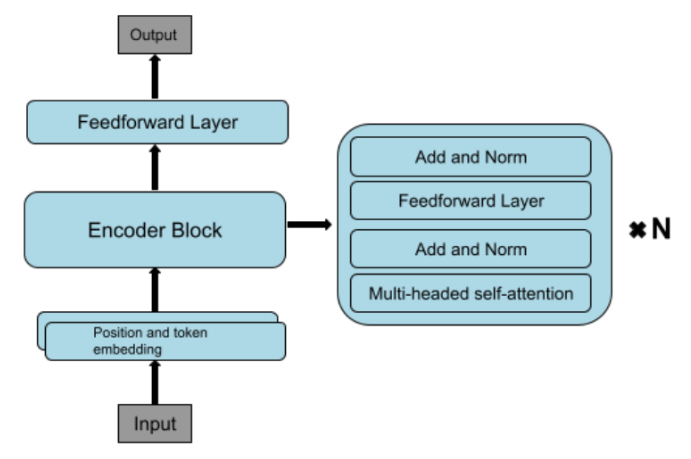
\includegraphics[width=0.95\linewidth]{drawing.png}
    \caption{Transformer Model}
    \label{fig:drawing}
\end{figure}

The multi-headed self-attention allows for the model to get context from other tokens in the sequence. It does this by computing attention scores between each token and the other tokens. Each head of self-attention is supposed to attend to a different part of the sequence, and they all come together to form one attention output. Our transformer also has a causal attention mask, which ensures that during training and predictions, the model can only attend to the past tokens in the sequence, and not the future tokens. This effectively stops the model from cheating, by not allowing it to use the context of the future tokens. In addition, the model also has a padding mask, that is applied during the loss calculation and during attention so that the model ignores the padding tokens.

\subsection{Fine-tuning}
\label{here}
We decided to try to keep our model dimensions similar, to keep the comparison between the two models unbiased. This means our embedding layer for both models was the same at 512 and both had a dropout of 0.1. In addition, both our models used cross-entropy loss, with Adam as the optimizer \cite{adam}. This only left us with a few parameters to fine-tune, leading us to decide on grid search as our method for fine-tuning the model.

For the LSTM we fine-tuned the number of layers and the learning rate. The exact values that we used for the grid search are shown in Table~\ref{tab:hyperl}.

\begin{table}[H]
    \centering
    \caption{Grid Search Values for LSTM}
    \label{tab:hyperl}
    \begin{tabularx}{\columnwidth}{X c c c} 
        \toprule
        \textbf{Hyperparameters} & \textbf{Values} \\ 
        \midrule
 Layers & 2, 3, 4, 6 \\
 Learning Rate & $1 \times 10^{-3}$, $1 \times 10^{-4}$, $5 \times 10^{-4}$  \\
        \bottomrule
    \end{tabularx}
\end{table}


The results of the grid search are in Table~\ref{tab:tab1} and Table~\ref{tab:tab2}. 

\begin{table}[ht]
    \centering
    \begin{tabular}{|c|c|c|c|}
    \hline
    \textbf{Layers/LR} & $1 \times 10^{-3}$ & $1 \times 10^{-4}$ & $5 \times 10^{-4}$ \\
    \hline
 2 & 78.14 & 78.01 & 78.41 \\
 3 & 77.90 & 77.44 & 78.06 \\
 4 & 72.42 & 77.01 & 77.63 \\
 6 & 67.00 & 75.63 & 72.48 \\
    \hline
    \end{tabular}
    \caption{Validation Accuracy for Different Hyperparameters}
    \label{tab:tab1}
\end{table}
    

\begin{table}[ht]
    \centering
    \begin{tabular}{|c|c|c|c|}
    \hline
    \textbf{Layers/LR} & $1 \times 10^{-3}$ & $1 \times 10^{-4}$ & $5 \times 10^{-4}$ \\
    \hline
 2 & 7.60  & 5.28 & 6.23 \\
 3 & 7.26  & 5.47 & 6.76 \\
 4 & 10.30 & 5.67 & 6.60 \\
 6 & 12.53 & 7.07 & 10.10 \\
    \hline
    \end{tabular}
    \caption{Validation Perplexity for Different Hyperparameters}
    \label{tab:tab2}
\end{table}
    

After completing the grid search for the LSTM we found the best model parameters were 2 layers with a learning rate of \(5\times10^{-4}\) resulting in the highest accuracy of 78.4\% and a perplexity of 6.23. Interestingly, the lowest perplexity was not from the model parameters that had the highest accuracy.

For the transformer, we fine-tuned the number of layers, which corresponds to the number of encoder blocks, the learning rate, and the dimension of the feedforward layer. The exact values we grid searched over can be found in Table~\ref{tab:hypert}.

\begin{table}[H]
    \centering
    \caption{Grid search values for Transformer.}
    \label{tab:hypert}
    \begin{tabular}{l c}
        \toprule
        \textbf{Hyperparameter} & \textbf{Values} \\
        \midrule
 Layers & 2, 4, 8 \\
 Learning Rate & \(1e{-3}\), \(1e{-4}\), \(1e{-5}\) \\
 Feedforward Dimension & 512, 1024, 2048 \\
        \bottomrule
    \end{tabular}
\end{table}

Some of the more interesting results can be found in Table~\ref{tab:tab3}. We did not report all of the 27 results.

\begin{table}[ht]
    \centering
    \begin{tabular}{|c|c|c|c|c|c|}
    \hline
    \textbf{Layers} & \textbf{LR} & \textbf{Dim FF} & \textbf{Accuracy} & \textbf{Perpl.} \\
    \hline
 2 & $1 e{-3}$ & 2048 & 0.9542 & 1.0003 \\
 4 & $1 e{-3}$ & 2048 & 0.9511 & 1.0003 \\
 4 & $1 e{-4}$ & 512  & 0.7869 & 1.0011 \\
 8 & $1 e{-3}$ & 2048 & 0.3883 & 1.0028 \\
 8 & $1 e{-4}$ & 512  & 0.7813 & 1.0011 \\
 8 & $1 e{-5}$ & 2048 & 0.5762 & 1.0022 \\
    \hline
    \end{tabular}
    \caption{Validation Accuracy and Test Perplexity for Selected Hyperparameter Settings}
    \label{tab:tab3}
\end{table}
    
Our fine-tuning resulted in the optimal model parameters being 2 layers, with a leading rate of \(1\times10^{-3}\), and a feedforward dimension of 2048. These hyperparameters achieved an accuracy of 95.42\% with a perplexity of 1.0003.

The main limitation of our fine-tuning was the time that the models took to train. The LSTM especially took a long time to train, leading to a smaller search grid.


\subsection{Evaluation}
We evaluated our models using two key metrics. The first evaluation was with next token prediction accuracy which is defined as the fraction of tokens that the model correctly predicts across all positions in the validation set. In addition, we also calculated the perplexity of both models, computed by exponentiating the average per-token loss:
\[
\exp\left(\frac{\text{total loss}}{\text{total tokens}}\right)
\]
The perplexity reflects how confidently the model assigns probability to the data. This is similar to what the two papers in the introduction papers did, however, the Microsoft Intellicode paper incorporated more metrics like ROGUE-L (Longest common subsequence) and edit similarity into their evaluation \cite{microsoft}.

%==================================================================================================================
%            Results
%==================================================================================================================

\section{Results}

After fine-tuning the parameters that were not kept constant between the two models, we can assume that each model is performing optimally. This is done to ensure that the comparison between the two models is as fair as possible. The following results for the models are with parameters determined from our hyperparameter tuning, which can be found above in Section~\ref{here}.


\subsection{Tokenizer}
We predicted that CodeBERT would outperform the GPT-2 and it did by a significant amount in the transformer. However, in the LSTM the difference in accuracy was minimal. The accuracy of the two different tokenizers for the transformer is shown in Figure~\ref{fig:toke}.

\begin{figure}[H]
    \centering
    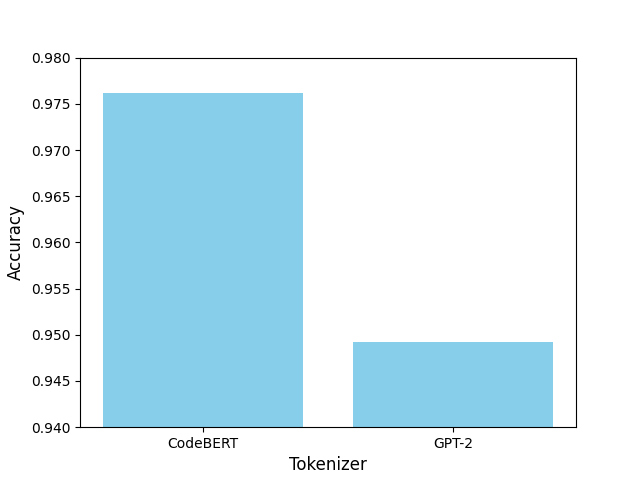
\includegraphics[width=0.95\linewidth]{bert_vs_gpt.png}
    \caption{CodeBERT Tokenizer vs GPT-2 Tokenizer}
    \label{fig:toke}
\end{figure}

CodeBERT had 2.7\% higher accuracy than when we used the GPT-2 tokenizer for the transformer. In addition, the perplexity was slightly lower as well, at 1.0001 and 1.0004 respectively. This is likely because CodeBERT was better able to tokenize the code into specific parts whereas, for some specific parts of the code, GPT-2 may have just labeled it as unknown. This is likely due to CodeBERT being trained specifically on code, while GPT-2's training was done on general plain text. The values in the following section, Section~\ref{rl} and Section~\ref{rt}, are using CodeBERT as the tokenizer.

\subsection{LSTM}
\label{rl}
On the held-out test set the LSTM had an accuracy of 78.51\% and a perplexity of 1.0004. The loss is shown below in Figure~\ref{fig:lossl}.

\begin{figure}[H]
    \centering
    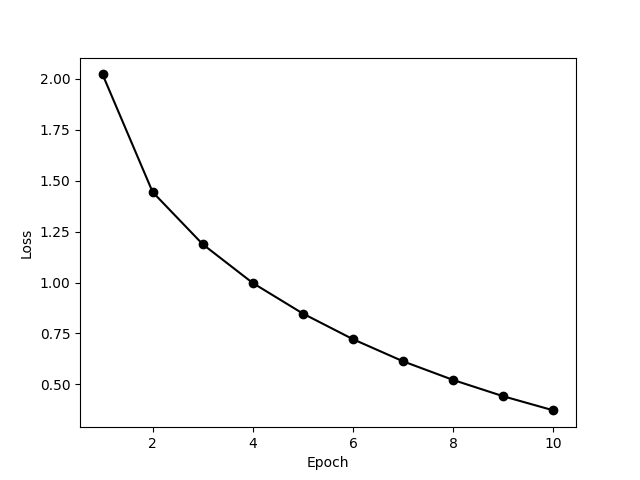
\includegraphics[width=0.95\linewidth]{lstm_loss.png}
    \caption{LSTM Loss}
    \label{fig:lossl}
\end{figure}

Over the ten epochs the LSTM was trained on, the loss, shown in Figure~\ref{fig:lossl} shows a smooth and gradual decline in average loss down to 0.3721. This indicates that it is consistently learning useful sequence patterns. Because the loss never goes up, it is clear that it is not overfitting just yet. If we ran it with even more epochs, it is likely that the loss would continue to go down. These loss values show that the LSTM is effectively capturing the long-range dependencies in the code and that extending the training loop could push the accuracy even higher.

\subsection{Transformer}
\label{rt}
On the held-out test set the transformer had an accuracy of 97.62\% and a perplexity of 1.0001. The loss is shown below in Figure~\ref{fig:losst}.

\begin{figure}[H]
    \centering
    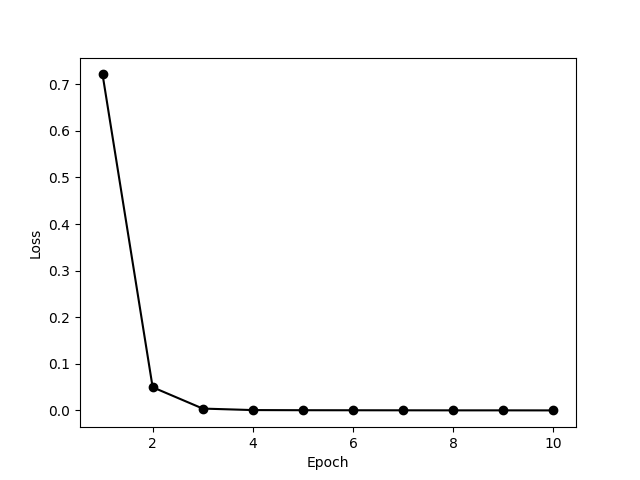
\includegraphics[width=0.95\linewidth]{trans_loss.png}
    \caption{Transformer Loss}
    \label{fig:losst}
\end{figure}

The transformer loss over the ten training epochs is very different from the LSTM. The loss drops off considerably at the start and goes down only slightly afterward. The bulk of the learning is happening within the first three epochs which tells us that the model is quickly fitting to the training set. After epoch four's loss of 0.0008, the loss only goes down by a fraction which is a sign of overfitting. To prevent overfitting we could have cut the model training off at three or four epochs, instead of ten to prevent overfitting, however, with more data the model may likely need those additional epochs.

\subsection{Comparison}
The transformer's higher accuracy and lower perplexity, as well as its efficiency in training, show that it is the superior option for code completion. This is due to the global context transformers have with their self-attention which can help capture context in code, such as a variable declared dozens of lines earlier. Its efficiency when training is due to the lack of recurrence and the ability to batch entire sequences in parallel. We can see the architectural advantages of the transformer when it fits the training data much faster than the LSTM and generalizes much better with its higher accuracy.


%==================================================================================================================
%            Conclusion
%==================================================================================================================

\section{Conclusion}
In this paper, we demonstrated that a Transformer-based architecture with CodeBERT tokenization outperforms a two-layer LSTM by over 16\% in accuracy. In addition, the loss converges significantly faster. We also showed that self-attention models capture long-range code dependencies far more effectively than an LSTM. The transformer's superior performance would make it ideal for real-world applications like a code completion app. Looking forward, we think it would be valuable to model multiple languages such as Java, Swift, and Go and train on significantly more data. Our results suggest that attention-based architectures present the most promising direction for code completion tools with the potential to allow developers to create software much more efficiently. 

%==================================================================================================================
%            Acknowledgements
%==================================================================================================================

\section{Acknowledgements}

This project used many Python packages. Many of these are cited in the text, but here is a complete list: Pytorch, TQDM, Transformers, Scikit-learn, and several modules from the Python standard library. Hugging Face was especially helpful, as we used it both for our models and tokenizers. This project was for a Natural Language Processing Class at Loyola Marymount University, and we received guidance and feedback that was crucial throughout the project from our instructor, Professor Mandy Korpusik. Finally, the paper style is from the ACL 2023 conference, and the template along with directions can be found here: \url{https://2023.aclweb.org/calls/style_and_formatting/}.

%==================================================================================================================
%            References
%==================================================================================================================

\nocite{*}
\bibliographystyle{plain}
\bibliography{Final_Paper}

\end{document}
